\documentclass{article}
\usepackage{amsfonts} 
\usepackage{amsmath}
\usepackage{hyperref}
\usepackage{graphicx}
\usepackage{subcaption}
\usepackage{booktabs}
\usepackage{makecell}
\usepackage{multirow}
%\usepackage{placeins}

\begin{document}


\section{Description}
\par The first we just calculated several Extended Barycentric Cubical Tori. The distribution of calculated toruses we can see in the Figure \ref{fig:cases_distribution}.
\begin{figure}[htbp]
    \centering
    \begin{subfigure}[t]{0.45\textwidth}
        \centering
        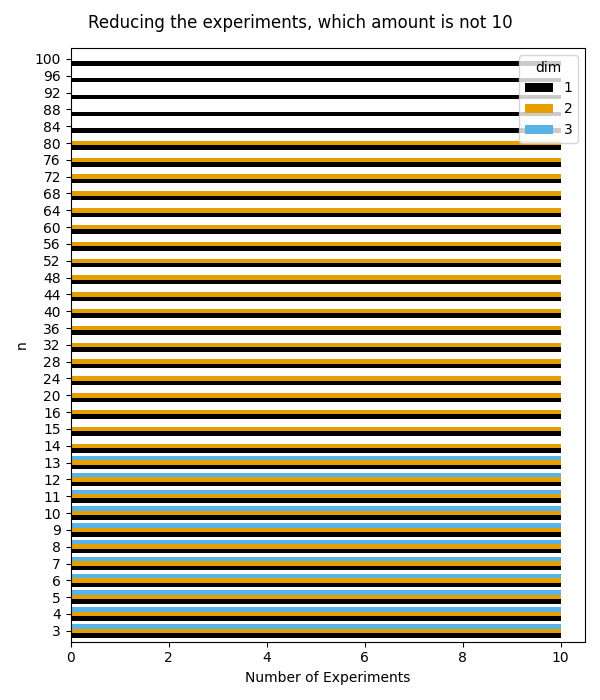
\includegraphics[width=\textwidth]{pics/extended torus scores/cases.png}
        \caption{Barycentric Cubical Tori}
        \label{fig:cases_distribution}
    \end{subfigure}
    \hfill
    \begin{subfigure}[t]{0.45\textwidth}
        \centering
        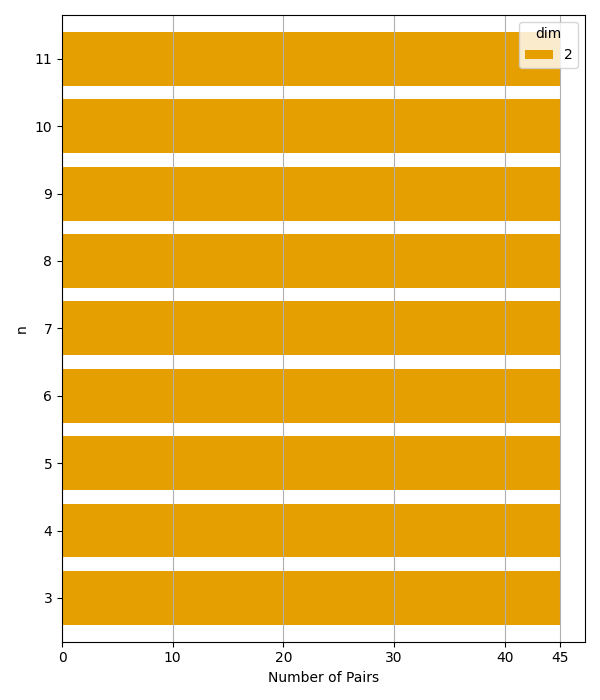
\includegraphics[width=\textwidth]{pics/torus-transpositions-extended/distribution.png}
        \caption{Calculated pairs}
        \label{fig:pairs_distribution}
    \end{subfigure}
    \caption{Size/dimension distribution}
    \label{fig:distribution}
\end{figure}

\par Then for each pair of filtrations with similar dimension and $n$ $f_0, f_1:\mathbb{T}^d_n \to \mathbb{R}$ we can define a linear homotopy $h: [0, 1]\times\mathbb{T}^d_n \to \mathbb{R}$:
$$
    h(t, \sigma) = (1 - t)\cdot f_0(\sigma) + t\cdot f_1(\sigma)
$$

\par The moment of time $t\in [0, 1]$ such there exist a pair of cells $\sigma_0, \sigma_1\in\mathbb{T}^d_n$ such that $h(t, \sigma_0) = h(t, \sigma_1)$ is a moment of transposition of these cells during the homotopy (the probability, that this will be full segment is 0 for pair of independent barycentric cubical tori).
\par We have found all transposing pairs like this, classified them and calculated how these transpositions cahnges the Depth Poset. The distribution of calculated pairs of filtration we can see in the Figure \ref{fig:pairs_distribution}.
\newpage

\section{Switch Types Distributions}

\par The distribution of transpositions types for the model $\mathbb{T}^{2}_n$ we can see in the figure Fig. \ref{fig:typesdistribution2}.
\begin{figure}[htbp]
\centering
\begin{subfigure}[b]{0.3\textwidth}
    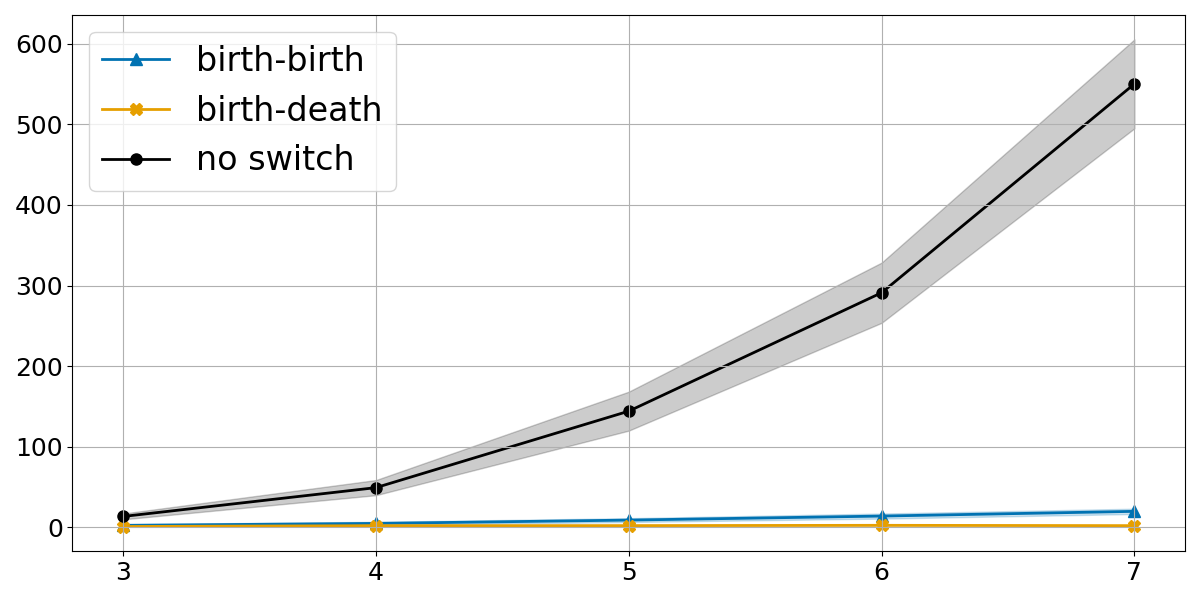
\includegraphics[width=\linewidth]{pics/torus-transpositions-extended/transposition-types-complex-dim2-subposet-dim0-drop-no-switches-False.png}
    \caption{Cells dimension 0}
    \label{fig:complex2cells0}
\end{subfigure}
\hfill
\begin{subfigure}[b]{0.3\textwidth}
    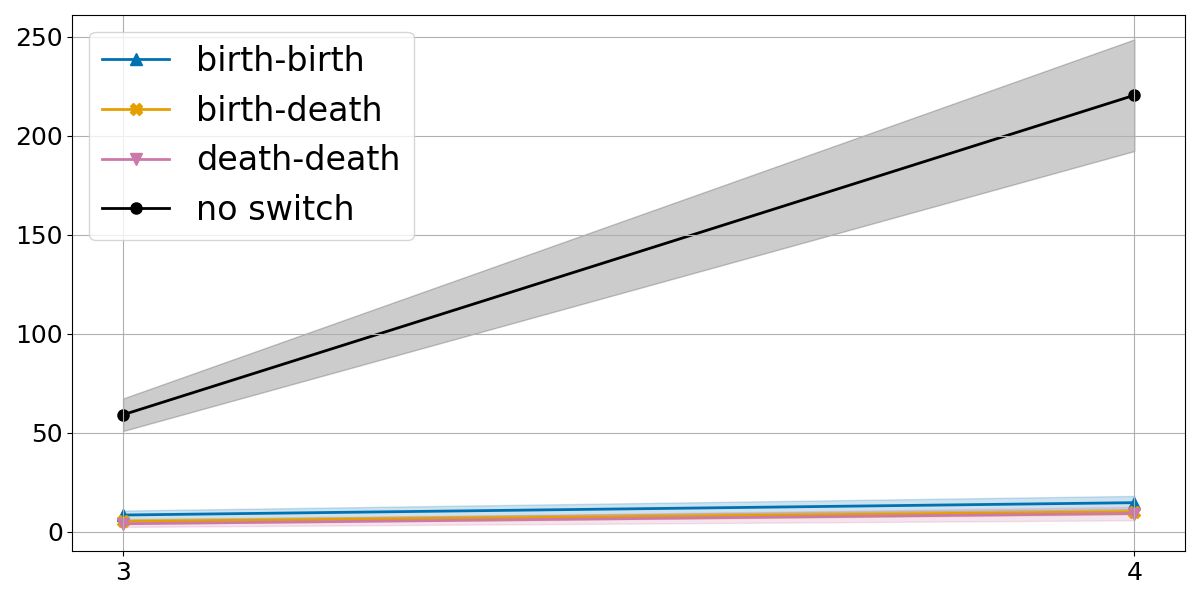
\includegraphics[width=\linewidth]{pics/torus-transpositions-extended/transposition-types-complex-dim2-subposet-dim1-drop-no-switches-False.png}
    \caption{Cells dimension 1}
    \label{fig:complex2cells1}
\end{subfigure}
\hfill
\begin{subfigure}[b]{0.3\textwidth}
    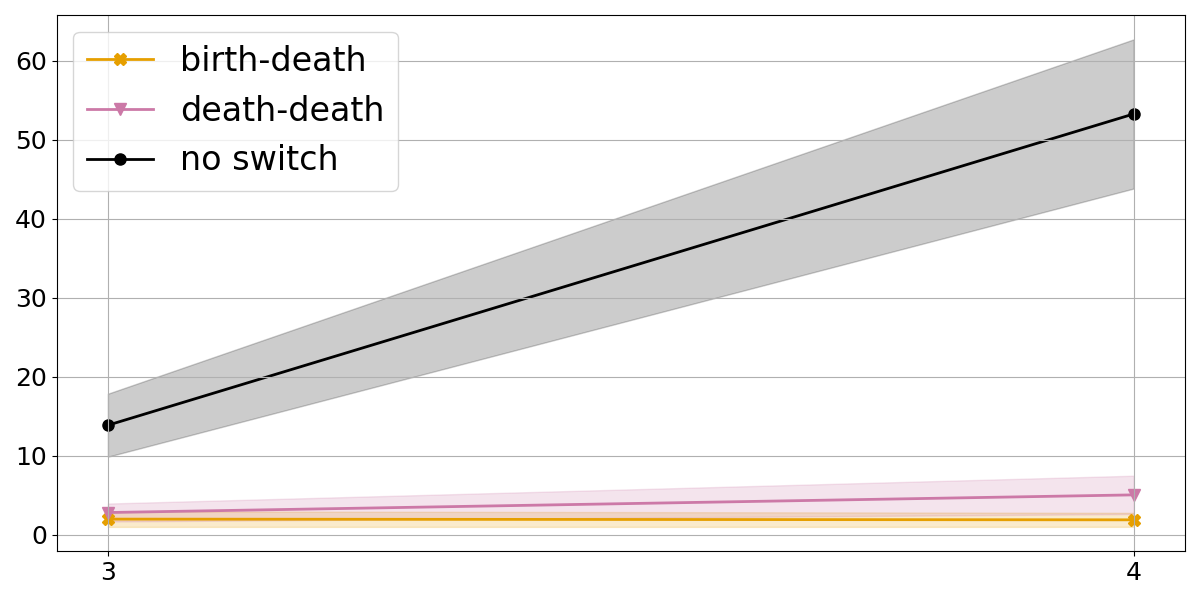
\includegraphics[width=\linewidth]{pics/torus-transpositions-extended/transposition-types-complex-dim2-subposet-dim2-drop-no-switches-False.png}
    \caption{Cells dimension 2}
    \label{fig:complex2cells2}
\end{subfigure}
\vspace{0.5cm}
\begin{subfigure}[b]{0.3\textwidth}
    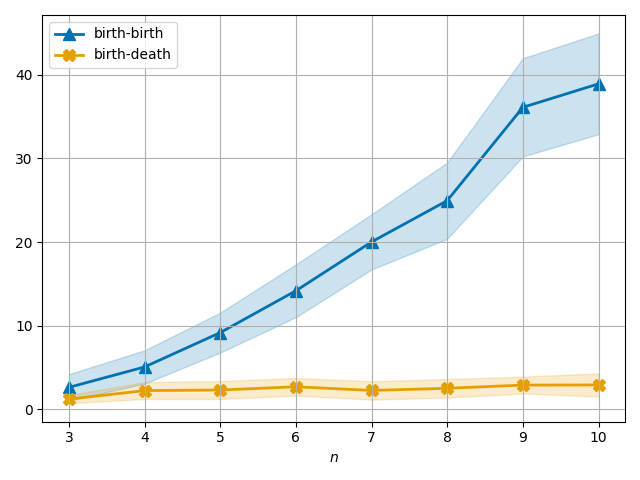
\includegraphics[width=\linewidth]{pics/torus-transpositions-extended/transposition-types-complex-dim2-subposet-dim0-drop-no-switches-True.png}
    \caption{Cells dimension 0 (without no switch transpositions)}
    \label{fig:complex2cells0onlyswitch}
\end{subfigure}
\hfill
\begin{subfigure}[b]{0.3\textwidth}
    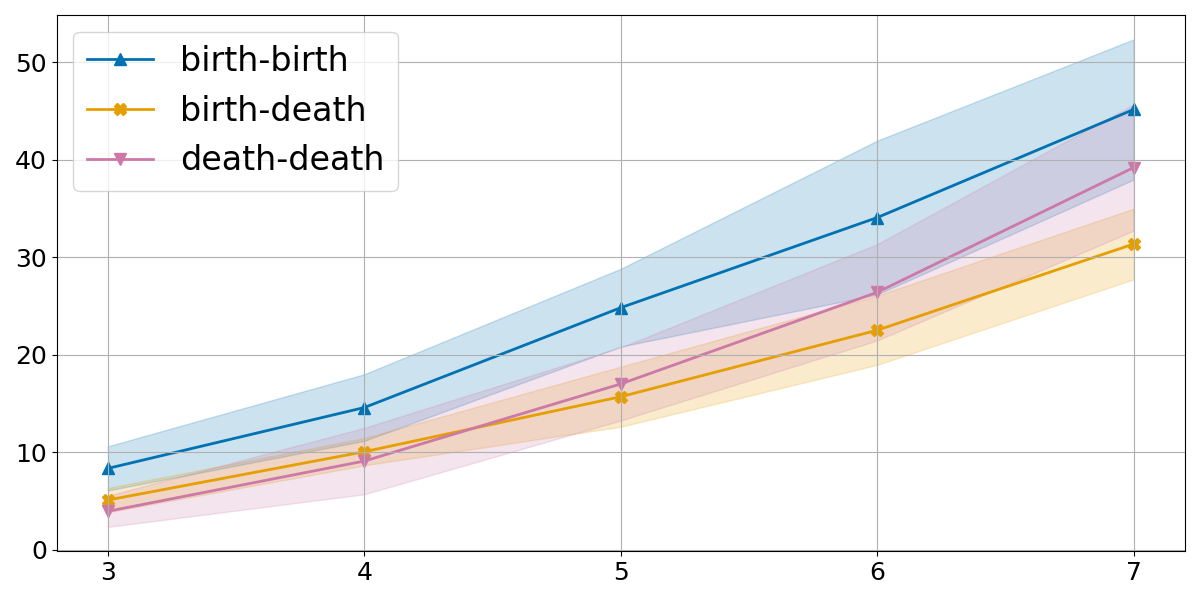
\includegraphics[width=\linewidth]{pics/torus-transpositions-extended/transposition-types-complex-dim2-subposet-dim1-drop-no-switches-True.png}
    \caption{Cells dimension 1 (without no switch transpositions)}
    \label{fig:complex2cells1onlyswitch}
\end{subfigure}
\hfill
\begin{subfigure}[b]{0.3\textwidth}
    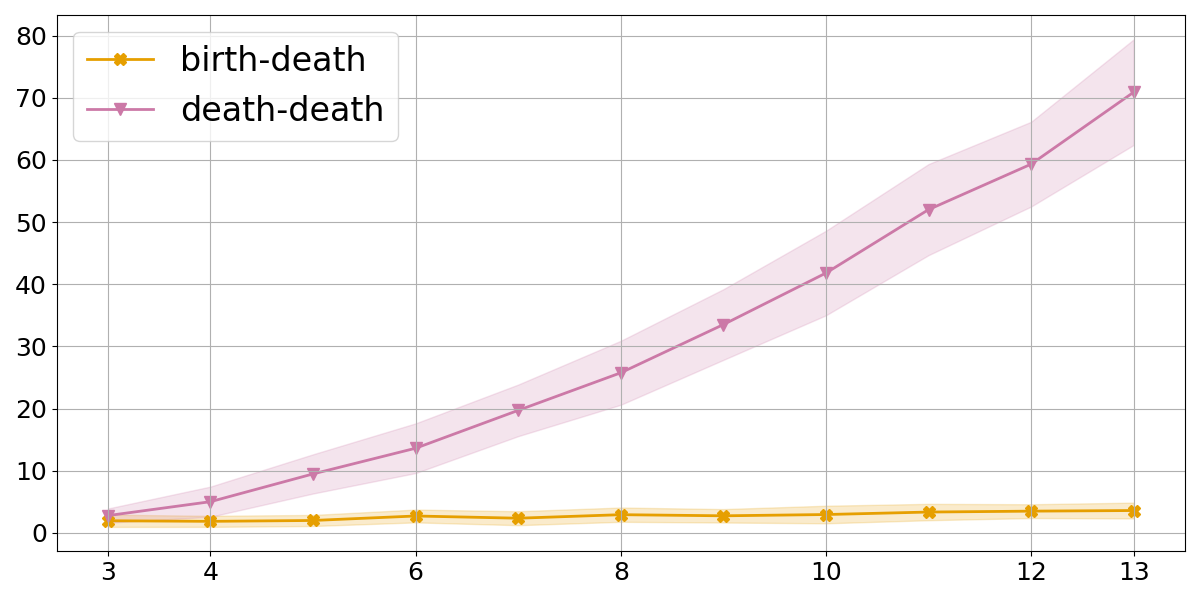
\includegraphics[width=\linewidth]{pics/torus-transpositions-extended/transposition-types-complex-dim2-subposet-dim2-drop-no-switches-True.png}
    \caption{Cells dimension 2 (without no switch transpositions)}
    \label{fig:complex2cells2onlyswitch}
\end{subfigure}
\caption{The switch type distribution for $\mathbb{T}_n^{2}$}
\label{fig:typesdistribution2}
\end{figure}
\newpage

\section{Similarity Scores}

\begin{itemize}
\item \textbf{birth\_relation\_cell\_similarity} - The size of symmetric difference of arcs (edges) in the birth relation (given by row left to right reduction algorithm).
    Consider 2 birth-death pairs are similar if they corespond the similar cells.
\item \textbf{death\_relation\_cell\_similarity} - The size of symmetric difference of arcs (edges) in the death relation (given by column bottom to top reduction algorithm).
    Consider 2 birth-death pairs are similar if they corespond the similar cells.
\item \textbf{poset\_closure\_arcs\_cell\_similarity} - The size of symmetric difference of arcs (edges) in the transitive closure of the Depth Posets.
    Consider 2 birth-death pairs are similar if they corespond the similar cells.
\item \textbf{poset\_reduction\_arcs\_cell\_similarity} - The size of symmetric difference of arcs (edges) in the transitive reduction of the Depth Posets.
    Consider 2 birth-death pairs are similar if they corespond the similar cells.
\end{itemize}
\par The distribution of the similarity scores for different models $\mathbb{T}^{dim}_n$ we can see in the following figures:
\begin{center}
\begin{tabular}{ll}
\toprule
dim & 2 \\
\midrule
birth\_relation\_cell\_similarity & Fig. \ref{fig:birthrelationcellsimilaritycomplex2} \\
death\_relation\_cell\_similarity & Fig. \ref{fig:deathrelationcellsimilaritycomplex2} \\
poset\_closure\_arcs\_cell\_similarity & Fig. \ref{fig:posetclosurearcscellsimilaritycomplex2} \\
poset\_reduction\_arcs\_cell\_similarity & Fig. \ref{fig:posetreductionarcscellsimilaritycomplex2} \\
\bottomrule
\end{tabular}

\end{center}
\begin{figure}[htbp]
\centering
\begin{subfigure}[b]{0.3\textwidth}
    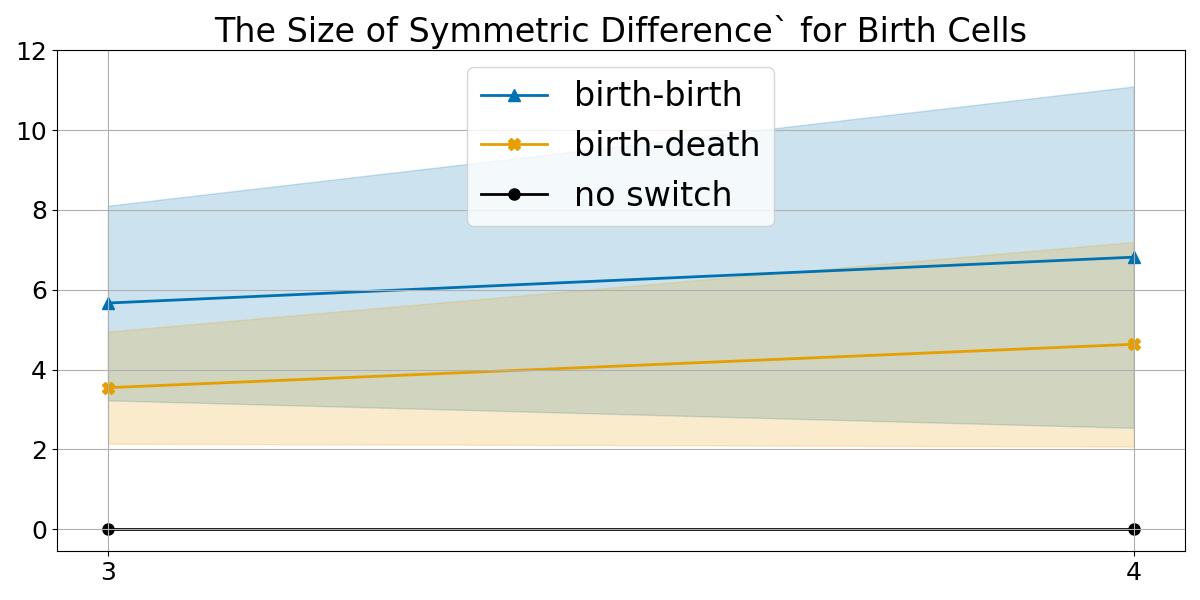
\includegraphics[width=\linewidth]{pics/torus-transpositions-extended/score-birth-relation-cell-similarity-complex-dim2-transpositions-dim0.png}
    \caption{Cells dimension 0}
    \label{fig:birthrelationcellsimilaritycomplex2cells0}
\end{subfigure}
\hfill
\begin{subfigure}[b]{0.3\textwidth}
    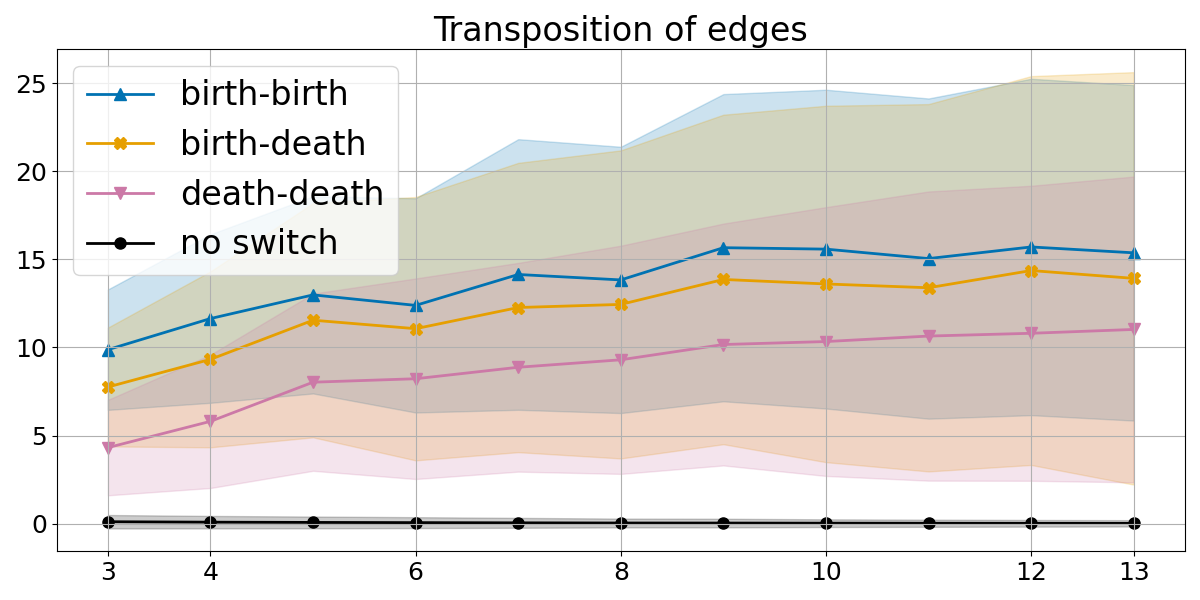
\includegraphics[width=\linewidth]{pics/torus-transpositions-extended/score-birth-relation-cell-similarity-complex-dim2-transpositions-dim1.png}
    \caption{Cells dimension 1}
    \label{fig:birthrelationcellsimilaritycomplex2cells1}
\end{subfigure}
\hfill
\begin{subfigure}[b]{0.3\textwidth}
    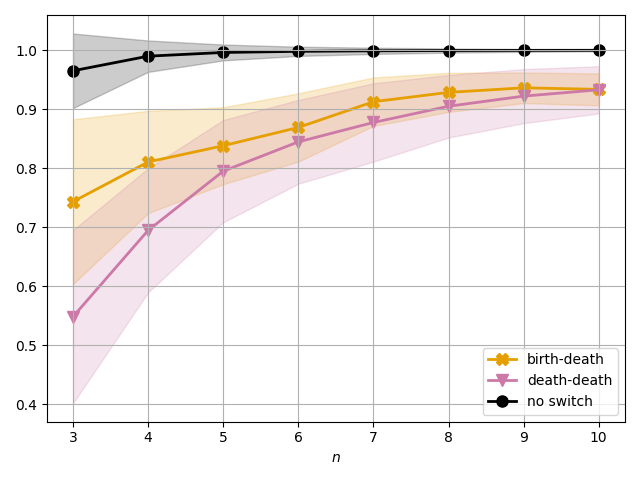
\includegraphics[width=\linewidth]{pics/torus-transpositions-extended/score-birth-relation-cell-similarity-complex-dim2-transpositions-dim2.png}
    \caption{Cells dimension 2}
    \label{fig:birthrelationcellsimilaritycomplex2cells2}
\end{subfigure}
\caption{Similarity score birth\_relation\_cell\_similarity for $\mathbb{T}_n^{2}$}
\label{fig:birthrelationcellsimilaritycomplex2}
\end{figure}

\begin{figure}[htbp]
\centering
\begin{subfigure}[b]{0.3\textwidth}
    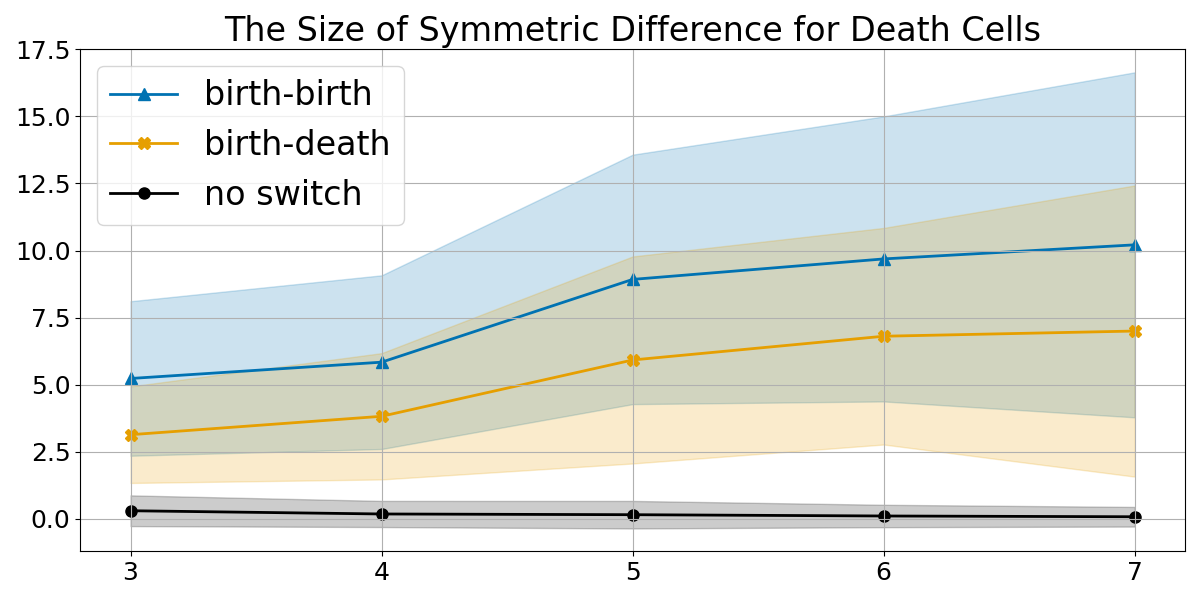
\includegraphics[width=\linewidth]{pics/torus-transpositions-extended/score-death-relation-cell-similarity-complex-dim2-transpositions-dim0.png}
    \caption{Cells dimension 0}
    \label{fig:deathrelationcellsimilaritycomplex2cells0}
\end{subfigure}
\hfill
\begin{subfigure}[b]{0.3\textwidth}
    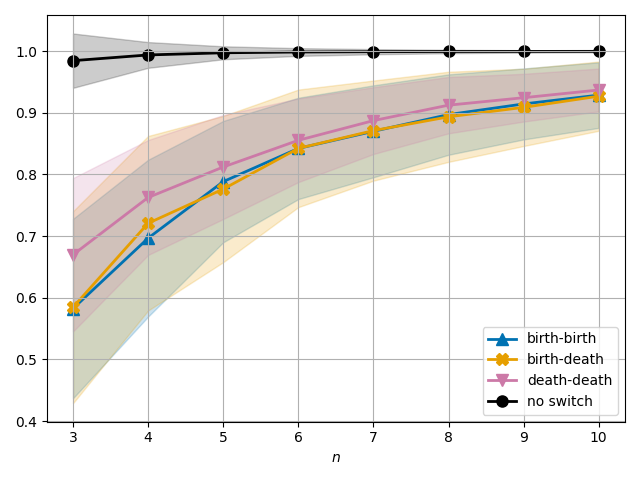
\includegraphics[width=\linewidth]{pics/torus-transpositions-extended/score-death-relation-cell-similarity-complex-dim2-transpositions-dim1.png}
    \caption{Cells dimension 1}
    \label{fig:deathrelationcellsimilaritycomplex2cells1}
\end{subfigure}
\hfill
\begin{subfigure}[b]{0.3\textwidth}
    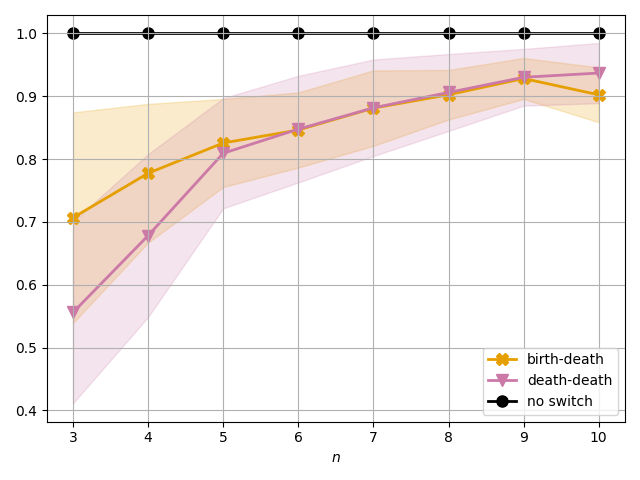
\includegraphics[width=\linewidth]{pics/torus-transpositions-extended/score-death-relation-cell-similarity-complex-dim2-transpositions-dim2.png}
    \caption{Cells dimension 2}
    \label{fig:deathrelationcellsimilaritycomplex2cells2}
\end{subfigure}
\caption{Similarity score death\_relation\_cell\_similarity for $\mathbb{T}_n^{2}$}
\label{fig:deathrelationcellsimilaritycomplex2}
\end{figure}

\begin{figure}[htbp]
\centering
\begin{subfigure}[b]{0.3\textwidth}
    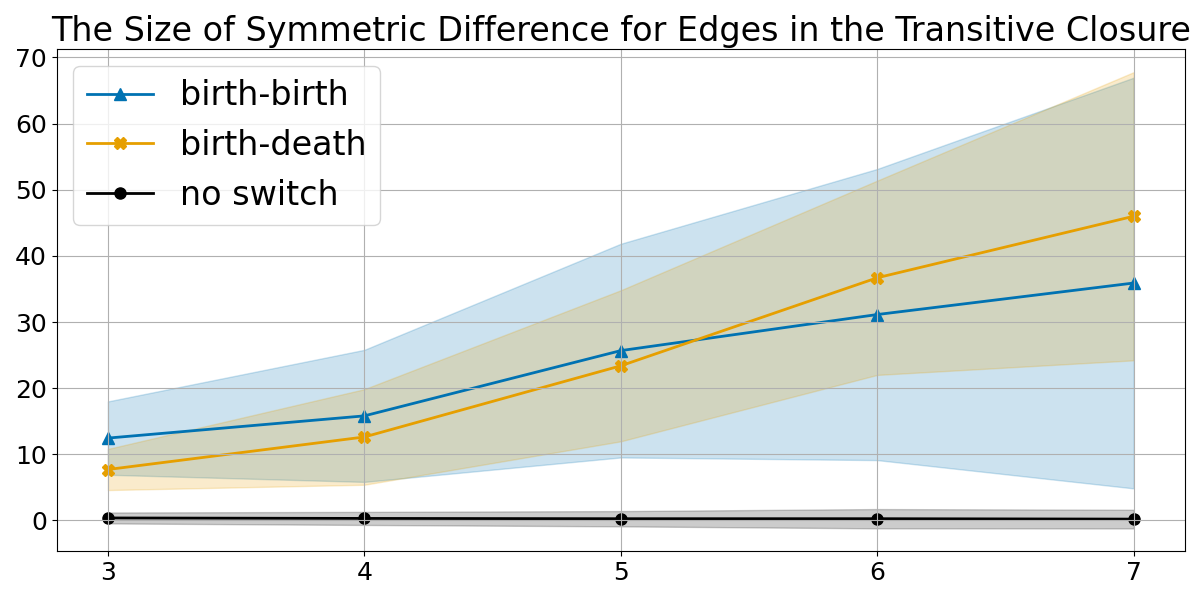
\includegraphics[width=\linewidth]{pics/torus-transpositions-extended/score-poset-closure-arcs-cell-similarity-complex-dim2-transpositions-dim0.png}
    \caption{Cells dimension 0}
    \label{fig:posetclosurearcscellsimilaritycomplex2cells0}
\end{subfigure}
\hfill
\begin{subfigure}[b]{0.3\textwidth}
    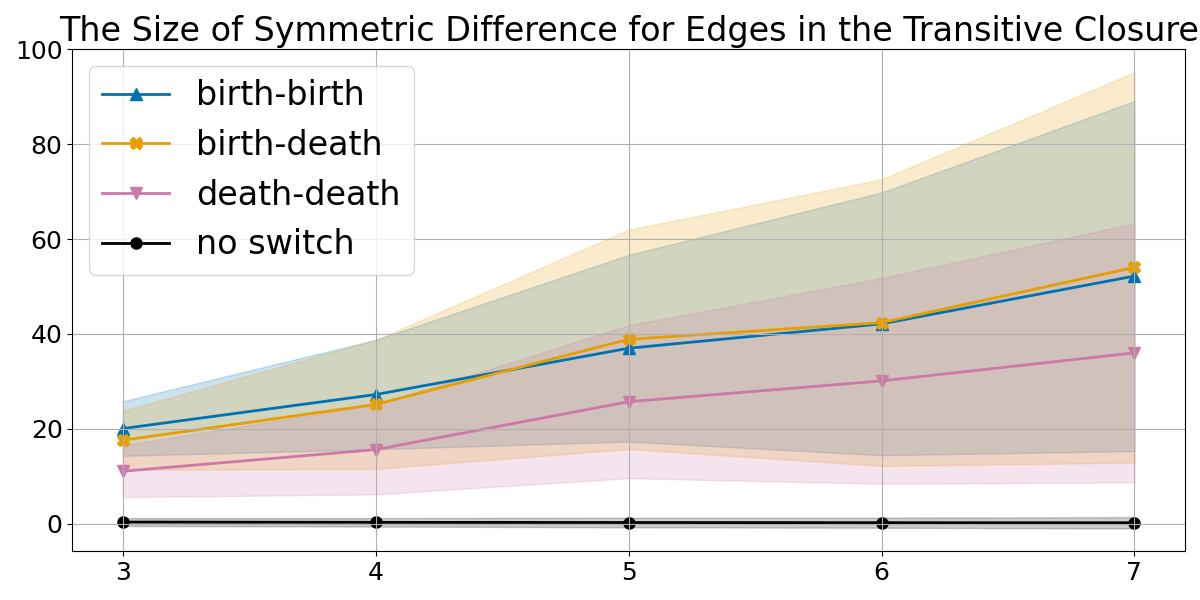
\includegraphics[width=\linewidth]{pics/torus-transpositions-extended/score-poset-closure-arcs-cell-similarity-complex-dim2-transpositions-dim1.png}
    \caption{Cells dimension 1}
    \label{fig:posetclosurearcscellsimilaritycomplex2cells1}
\end{subfigure}
\hfill
\begin{subfigure}[b]{0.3\textwidth}
    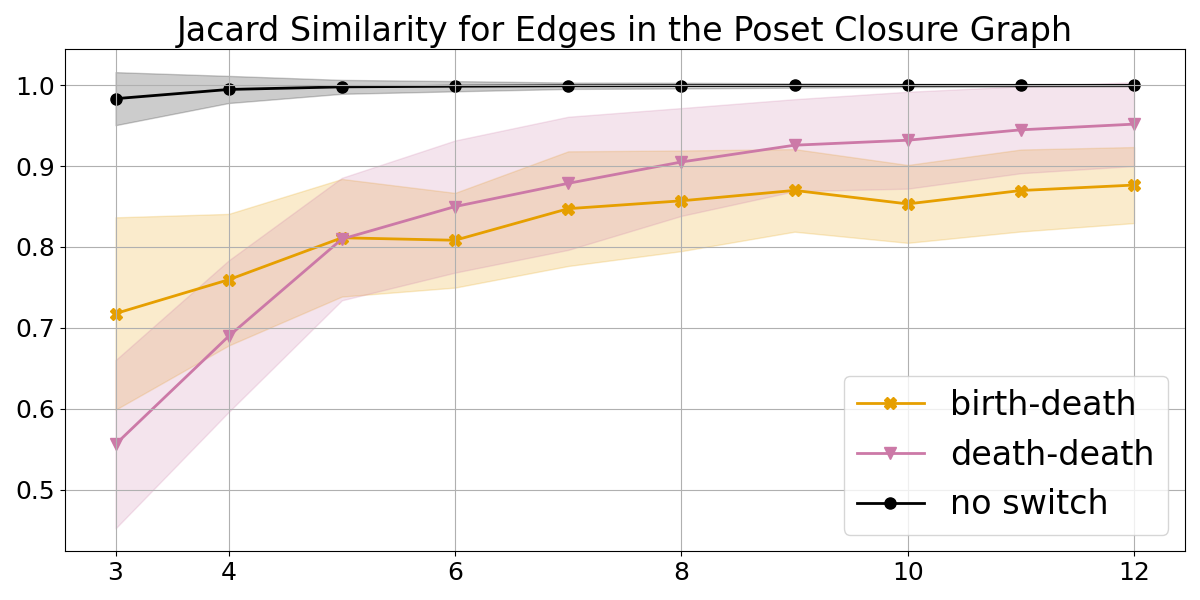
\includegraphics[width=\linewidth]{pics/torus-transpositions-extended/score-poset-closure-arcs-cell-similarity-complex-dim2-transpositions-dim2.png}
    \caption{Cells dimension 2}
    \label{fig:posetclosurearcscellsimilaritycomplex2cells2}
\end{subfigure}
\caption{Similarity score poset\_closure\_arcs\_cell\_similarity for $\mathbb{T}_n^{2}$}
\label{fig:posetclosurearcscellsimilaritycomplex2}
\end{figure}

\begin{figure}[htbp]
\centering
\begin{subfigure}[b]{0.3\textwidth}
    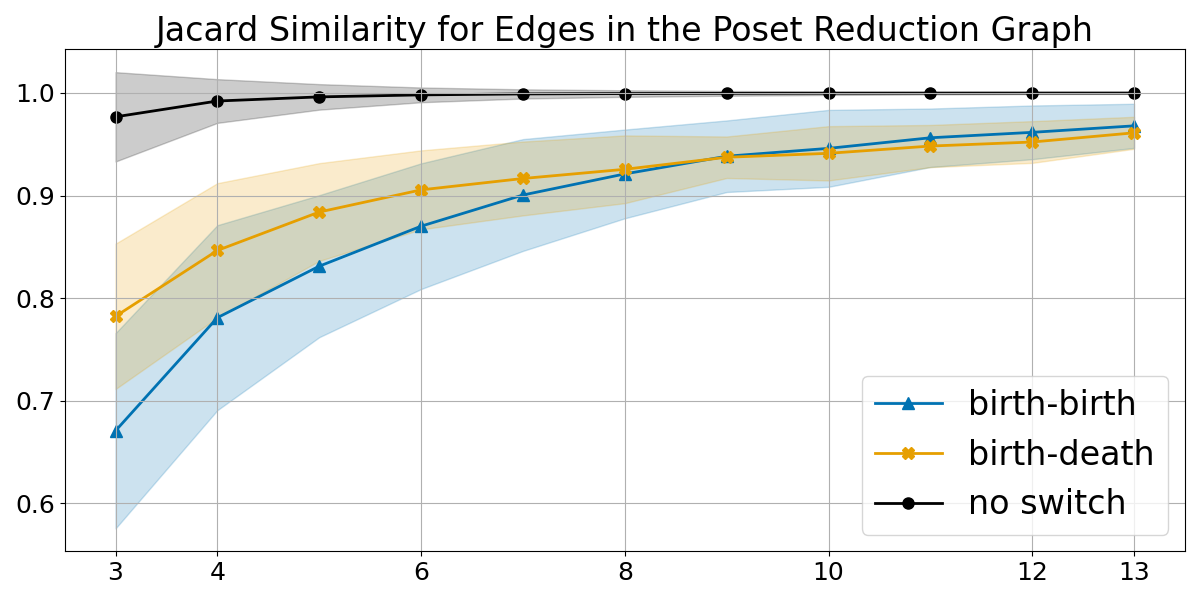
\includegraphics[width=\linewidth]{pics/torus-transpositions-extended/score-poset-reduction-arcs-cell-similarity-complex-dim2-transpositions-dim0.png}
    \caption{Cells dimension 0}
    \label{fig:posetreductionarcscellsimilaritycomplex2cells0}
\end{subfigure}
\hfill
\begin{subfigure}[b]{0.3\textwidth}
    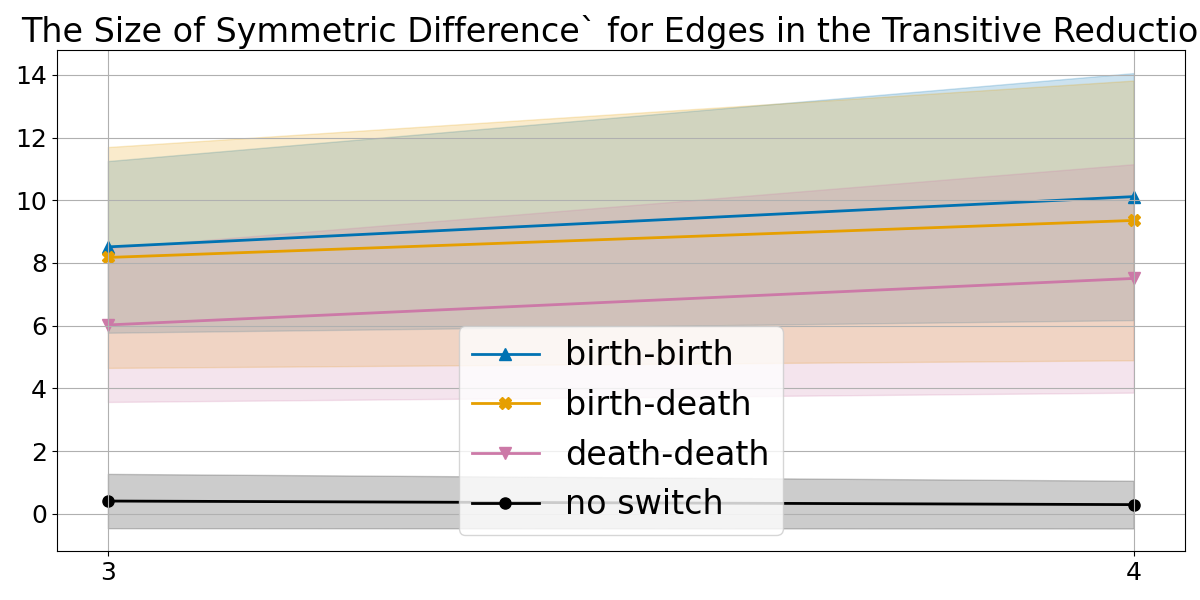
\includegraphics[width=\linewidth]{pics/torus-transpositions-extended/score-poset-reduction-arcs-cell-similarity-complex-dim2-transpositions-dim1.png}
    \caption{Cells dimension 1}
    \label{fig:posetreductionarcscellsimilaritycomplex2cells1}
\end{subfigure}
\hfill
\begin{subfigure}[b]{0.3\textwidth}
    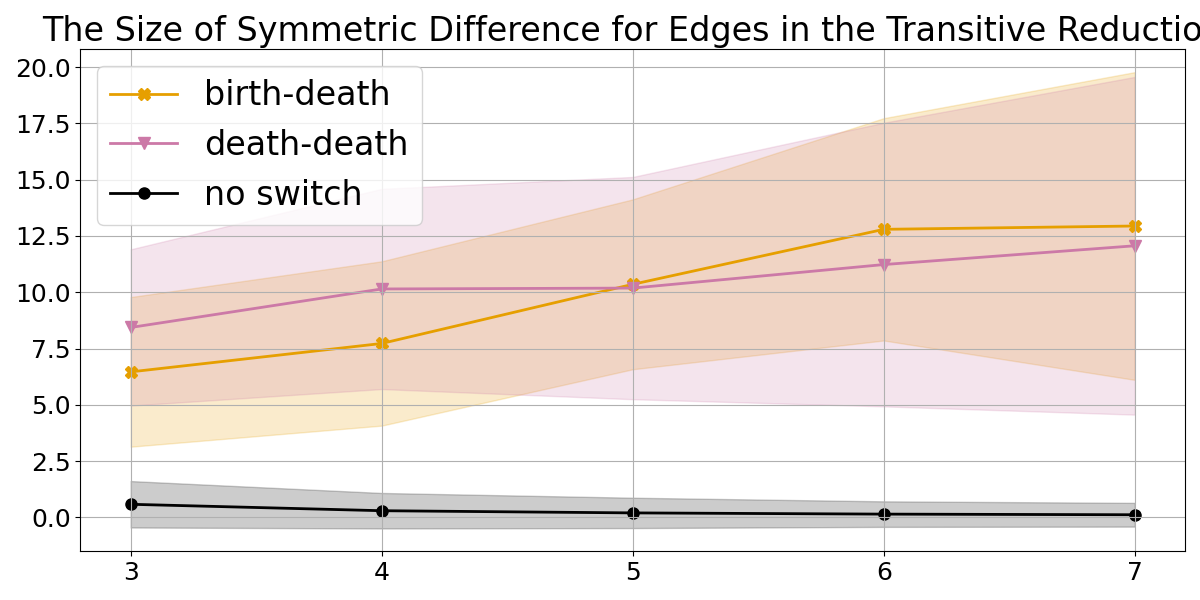
\includegraphics[width=\linewidth]{pics/torus-transpositions-extended/score-poset-reduction-arcs-cell-similarity-complex-dim2-transpositions-dim2.png}
    \caption{Cells dimension 2}
    \label{fig:posetreductionarcscellsimilaritycomplex2cells2}
\end{subfigure}
\caption{Similarity score poset\_reduction\_arcs\_cell\_similarity for $\mathbb{T}_n^{2}$}
\label{fig:posetreductionarcscellsimilaritycomplex2}
\end{figure}




\end{document}